%----------createStereotype----------------------------------------
\op
{createStereotype}
{creates a new stereotype}
{createStereotype(Package selectedEObject, String nameValue)}
{The model providing the container for the newly created stereotype.}
{
\begin{itemize}
 \item nameValue/newName: The name of the newly created stereotype
 \item idValue/newID: The id of the newly created stereotype
\end{itemize}
}
{There is no stereotype whose name equals the parameter-value of 'newName' (see
\ref{subsec:checkOtherNames})}
{Only the name and the id will be set via input data.}
\begin{figure}[H]
  \centering
  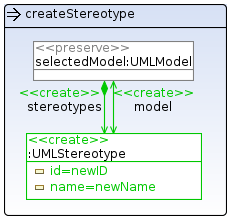
\includegraphics[width=0.4\textwidth]{pics/createStereotype.png}
  \caption{createStereotype}
  \label{createStereotype}
\end{figure}
%----------deleteStereotype----------------------------------------
\op
{deleteStereotype}
{Deletes a stereotype}
{deleteStereotype(Stereotype selectedEObject)}
{The stereotype which should be deleted}
{-}
{-}
{For a better readability this is a simplified version of the
'deleteStereotype'-transformation and will only cover cases where the stereotype
has no containments and no references to other elements. Such a complex
transformation rule exits but won't be listed here.}
\begin{figure}[H]
  \centering
  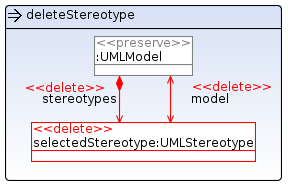
\includegraphics[width=0.4\textwidth]{pics/deleteStereotype_emptyAndUnreferenced.png}
  \caption{deleteStereotype}
  \label{deleteStereotype}
\end{figure}
%----------editStereotypeName----------------------------------------
\op
{editStereotypeName}
{edits the name of a stereotype}
{editStereotypeName(Stereotype selectedEObject, String nameValue)}
{The stereotype whose name should be renamed.}
{
\begin{itemize}
 \item nameValue/newName: The new name
\end{itemize}
}
{There is no stereotype in the same package whose name equals the parameter-value of
'newName' (see
\ref{subsec:checkOtherNames})}
{The \textless\textless create\textgreater\textgreater  -symbol in the image
means that even if the attribute exists its value will be overwritten.
'newName' is the placeholder for the input name.}
\begin{figure}[H]
  \centering
  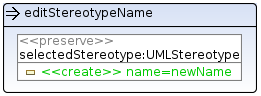
\includegraphics[width=0.4\textwidth]{pics/editStereotypeName.png}
  \caption{editStereotypeName}
  \label{editStereotypeName}
\end{figure}